\documentclass[../report.tex]{subfiles}

\begin{document}
\subsection{Định nghĩa và khái niệm}
Các khái niệm: 
\begin{itemize}
\item Điểm biên: Một điểm ảnh được coi là điểm biên 
nếu có sự thay đổi nhanh hoặc đột ngột về mức xám (hoặc màu). 
Ví dụ trong ảnh nhị phân, điểm đen gọi là điểm biên 
nếu lân cận nó có ít nhất một điểm trắng.  \cite{slide} \cite{bookhvbc}

\item Đường biên (đường bao - boundary): Tập hợp các 
điểm biên liên tiếp tạo thành một đường biên hay đường bao.  
\end{itemize}

\noindent Ý nghĩa của đường biên trong xử lý: 
\begin{itemize}
\item Đường biên là một loại đặc trưng cục bộ tiêu biểu 
trong phân tích, nhận dạng ảnh. 
\item Được sử dụng làm phân cách các vùng xám (màu) cách biệt. 
\end{itemize}

\noindent Tuy nhiên ngược lại, người ta cũng 
sử dụng các vùng ảnh để tìm đường phân cách.

Mô hình biểu diễn đường biên theo toán học: Điểm ảnh có sự biến đổi mức xám u(x) một cách đột ngột theo hình dưới. 
\begin{figure}[H]
\centering
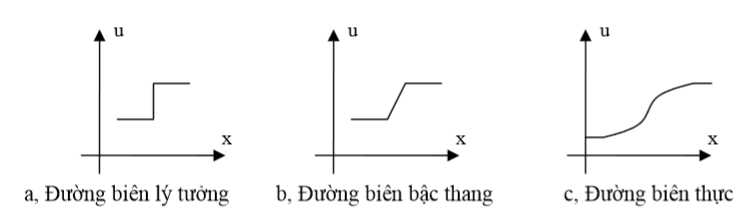
\includegraphics[width=\textwidth]{figures/edges.png}
\caption{Đường bao của ảnh}
\end{figure}

\subsection{Các kỹ thuật phát hiện biên}
Từ định nghĩa toán học của biên người ta sử dụng 
hai phương pháp phát hiện biên như sau
\begin{itemize}
\item Phương pháp phát hiện biên trực tiếp: 
Phương pháp này chủ yếu dựa vào sự biến thiên 
độ sáng của điểm ảnh để làm nổi biên bằng kỹ thuật đạo hàm.
\begin{itemize}
\item Nếu lấy đạo hàm bậc nhất của ảnh: Ta có phương pháp Gradient
\item Nếu lấy đạo hàm bậc hai của ảnh: Ta có phương pháp Laplace. 
\end{itemize}
Hai phương pháp này được gọi chung là phương pháp 
dò biên cục bộ. Ngoài ra, người ta còn sử dụng phương 
pháp “đi theo đường bao” dựa vào công cụ toán học 
là nguyên lý quy hoạch động và đượng gọi là phương 
pháp dò biên tổng thể. Phương pháp dò biên trực tiếp 
có hiệu quả và ít bị tác động của nhiễu.

\item Phương pháp phát hiện biên gián tiếp: 
Nếu bằng cách nào đấy, chúng ta thu đượng các 
vùng ảnh khác nhau thì đường phân cách giữa các 
vùng đó chính là biên. Nói cách khác, 
việc xác định đường bao của ảnh được thực hiện từ ảnh đã được 
phân vùng. Phương pháp dò biên gián tiếp khó cài 
đặt nhưng áp dụng tốt khi sự biến thiên độ sáng nhỏ. 
\end{itemize}
\emph{Chú ý:} Kỹ thuật dò biên và phân vùng ảnh là hai bài 
toán đối ngẫu của nhau. 

\subsection{Quy trình phát hiện biên}
\begin{itemize}
\item B1: Do ảnh ghi được thường có nhiễu, bước một là phải lọc nhiễu theo các phương pháp dã tìm hiểu ở các phần trước.

\item B2: Làm nổi biên sử dụng các toán tử phát hiện biên. 

\item B3: Định vị biên. Chú ý rằng kỹ thuật nổi biên 
    gây tác dụng phụ là gây nhiễu làm một 
    số biên giả xuất hiện do vậy cần loại bỏ biên giả. 
\item B4: Liên kết và trích chọn biên. 
\end{itemize}

\subsection{Phương pháp Gradient}
Theo định nghĩa về Gradient, nếu áp dụng nó vào xử lý ảnh, 
việc tính toán sẽ rất phức tạp. Để đơn giản mà không 
mất tính chất của phương pháp Gradient, người ta sử 
dụng kỹ thuật Gradient dùng cặp mặt nạ $H_1$, 
$H_2$ trực giao (theo 2 hướng vuông góc). Nếu định nghĩa 
$g_1$, $g_2$ là Gradient theo hai hướng $x$, $y$ tướng ứng thì 
biên độ $g(m,n)$ tại điểm $(m, n)$ được tính: 
\begin{align*}
g(m, n) &= \sqrt{g_1^2(m, n) + g_2^2(m, n)} = A_0 \\
\theta_r(m, n) &= \arctan \left(\frac{g_2(m, n)}{g_1(m, n)}\right)
\end{align*}
Để giảm độ phức tạp tính toán, $A_0$ được tính gần đúng như sau:
\begin{align*}
A_0 &= |g_1(m, n)| + |g_2(m, n)|
\end{align*}

\subsubsection{Toán tử Robert (1965)}
Với mỗi điểm ảnh $I(x,y)$ đạo hàm theo $x$, $y$ 
được các giá trị tương ứng $g_x$, $g_y$:
\begin{align*}
g_x &= I(x + 1, y) - I(x, y + 1) \\
g_y &= I(x + 1, y + 1) - I(x, y)
\end{align*}
Các công thức kể trên được cụ thể hóa bằng 
các mặt nạ theo chiều $x$ và $y$ tương ứng như sau:
\begin{figure}[H]
\centering
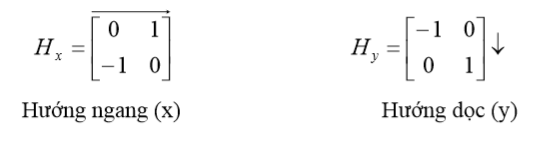
\includegraphics[width=9cm]{figures/sobert-operator.png}
\end{figure}
 
\subsubsection{Toán tử Sobel}
Toán tử Sobel được Duda và Hart đặt ra năm 
1973 với các mặt nạ tương tự như của 
Robert nhưng cấu hình khác như sau:
\begin{figure}[H]
\centering
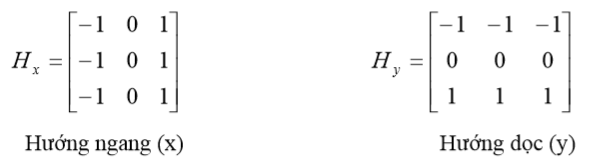
\includegraphics[width=10cm]{figures/sobel-operator.png}
\end{figure}

\subsubsection{Toán tử Prewitt}
Toán tử được Prewitt đưa ra vào năm 1970 có dạng:
\begin{figure}[H]
\centering
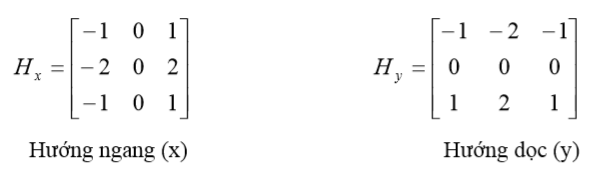
\includegraphics[width=10cm]{figures/prewitt-operator.png}
\end{figure}

\subsection{Nhận xét các phương pháp Gradient}
\begin{itemize}
\item Toán tử Prewitt có thể tách sườn đứng tốt hơn toán tử Sobel, 
trong khi đó toán tử Sobel tách các sườn trên các điểm ở 
đường chéo tốt hơn.

\item Toán tử Robert nhược điểm là nhạy với nhiễu.

\item Để đạt được kết quả mong muốn các toán tử Gradient 
    thường được dùng trước để làm sạch nhiễu.

\item Các mặt nạ của các toán tử trên có kích 
thước $2 \times 2$ hoặc $3 \times 3$ chiều. 
Các mặt nạ có số chiều lớn hơn cũng được sử dụng. 
Ví dụ trong kỹ thuật phát hiện biên người ta dùng mặt 
nạ $5 \times 5$ cho toán tử Sobel:
\begin{figure}[H]
\centering
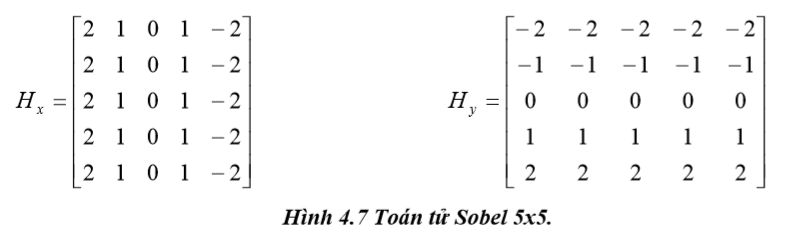
\includegraphics[width=12cm]{figures/sobel-5x5.png}
\end{figure}

\item Các toán tử kể trên đều sử dụng các mặt nạ theo 
hai chiều $(x, y)$ tức là bốn hướng $(-x, y; -y, y)$.
\end{itemize}

\end{document}

